\section{Revisão Bibliográfica} \label{revisaobibliografica}

Redes Neurais Artificiais são técnicas computacionais que apresentam um modelo matemático inspirado na estrutura neural de organismos inteligentes e que adquirem conhecimento através da experiência. A arquitetura base de rede neural estudada neste artigo é a Perceptron de Múltiplas Camadas (do inglês, Multilayer Perceptron, ou apenas MLP) \cite{kovacs2002redes} \cite{haykin2007redes}.

\subsection{Perceptrom de Multiplas Camadas}

Uma rede MLP consiste em pelo menos três camadas: uma camada de entrada, uma camada oculta e uma camada de saída. O MLP utiliza uma técnica de aprendizado supervisionada chamada \textit{backpropagation} para o treinamento.

\begin{figure}[H]

\centering % para centralizarmos a figura
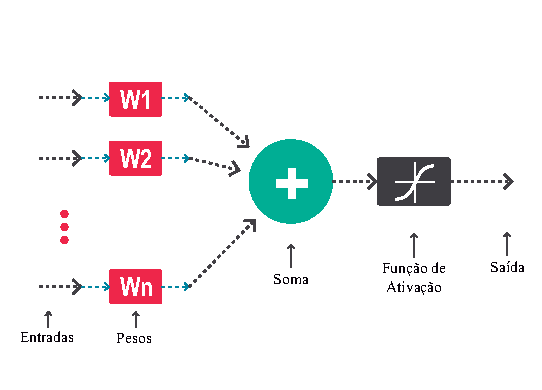
\includegraphics{04-Figuras/Arquitetura}

\caption{Arquitetura de uma rede MLP}

\label{figura:arquitetura}

\end{figure}

A rede é alimentada pela camada de entrada, de maneira que as entradas serão ponderadas por pesos e, logo em seguida, serão somados de submetidos a uma função de ativação (na camada intermediária). Por fim, após este processamento, haverá uma resposta na camada de saída da rede, como ilustra a fig. \ref{figura:arquitetura}.



\subsection{Algoritmo Backpropagation}


Quando verifica-se a resposta na camada de saída de uma MLP, podemos estimar o grau de acerto da rede. Portanto, há um valor esperado (e conhecido) para a resposta da rede durante a fase de treinamento. Logo, podemos extrair o erro dessa rede. O algoritmo \textit{backpropagation} visa realimentar o erro nas entradas com o objetivo de minimizá-lo ao máximo. Essa característica é chamada de retropropagação do erro \cite{kovacs2002redes}.

\subsection{Estrutura Competitiva Auto Associativa}

Redes neurais auto associativas são redes de \textit{feedforward} treinadas para produzir uma aproximação do mapeamento de identidade entre entradas e saídas da rede usando o algoritmo \textit{backpropagation} \cite{Miranda}.

\begin{figure}[H]

\centering % para centralizarmos a figura
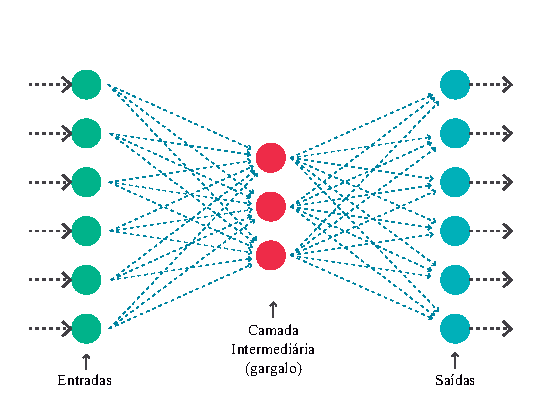
\includegraphics{04-Figuras/associativa}

\caption{Arquitetura de uma rede auto associativa}

\label{figura:associativa}

\end{figure}

O principal recurso de uma rede auto associativa é um gargalo dimensional entre entrada e saída (uma vez que as camadas de entrada e saída são as mesmas e o numero de neurônio na camada intermediária é inferior aos da entrada/saída). A compactação de informações pelo gargalo resulta na aquisição de um modelo de correlação dos dados de entrada, útil para executar uma variedade de tarefas de triagem de dados.


%=================================================================================================
%=================================================================================================

\section{Base de Dados} \label{baseDados}

A base de dados tratada neste trabalho é referente a 13 parâmetros (características) de três classes de vinho, onde totaliza 178 instâncias de dados coletados. Os parâmetros são resultados de uma análise química das três classes de vinhos, a saber: álcool, ácido málico, cinza, alcalinidade das cinzas, magnésio, fenóis totais, flavinóides, fenóis não-flavonóides, proantocianinas, intensidade de cor, matiz, OD280/OD315 de vinho diluídos e prolina \cite{fraley2007model}.





\begin{table}[H]
\centering
\caption{Distribuição da base de dados}
\resizebox{\columnwidth}{!}{%
\begin{tabular}{ccccc}
\hline
Classe & Treino & Validação & Teste & Total \\ \hline
1      & 39     & 10        & 10    & 59    \\
2      & 51     & 10        & 10    & 71    \\
3      & 28     & 10        & 10    & 48    \\ \hline
\end{tabular}%
}

\label{tabela:baseDados}

\end{table}



Das 178 instâncias 59 pertencem à classe 1, 71 pertencem à classe 2 e 48 à classe 3, como mostra a tabela \ref{tabela:baseDados}.



%=================================================================================================
%=================================================================================================


\section{Desenvolvimento da Rede MLP} \label{desenvolvimentoMLP}

A rede MLP foi implementada utilizando 13 neurônio na camada de entrada, 5 neurônio na camada intermediária e um neurônio na camada de saída.

A topologia da rede foi escolhida variando-se o número de neurônios na camada intermediária e fazendo um estudo sobre o erro médio quadrático (do inglês, MSE) e o número de erros na classificação.





\begin{table}[H]
\centering
\caption{Melhor topologia MLP}
\resizebox{\columnwidth}{!}{%
\begin{tabular}{ccc}
\hline
NEURÔNIOS & MSE                & ERROS \\ \hline
1         & 0.0705937829921329 & 3     \\
3         & 0.0630764717369302 & 2     \\
5         & 0.0157501702325207 & 1     \\
10        & 0.0779010995153948 & 1     \\
20        & 0.0883763713087734 & 2     \\
40        & 0.155451160809213  & 6     \\
80        & 0.158974910948916  & 5     \\ \hline
\end{tabular}%
}

\label{tabela:MLP_MSE}

\end{table}

							%->	Tabela 01

A tabela \ref{tabela:MLP_MSE} mostra o desempenho de cada topologia de rede MPL. Observa-se que o melhor desempenho foi obtido pela rede com 5 neurônios na camada intermediária, pois apresentou o menor erro médio quadrático e o menor número de erros na classificação.


\subsection{Arquitetura MLP}

\begin{figure}[H]

\centering % para centralizarmos a figura
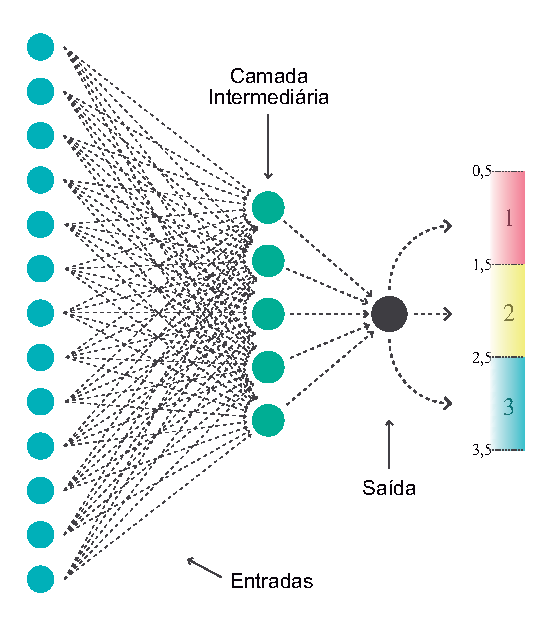
\includegraphics{04-Figuras/Arquitetura-MPL}

\caption{Arquitetura da rede MLP}

\label{figura:arquiteturaMPL}

\end{figure}


A fig. \ref{figura:arquiteturaMPL} mostra a arquitetura da rede MPL. As 13 entradas alimentam os 5 neurônios na camada intermediária e, por conseguinte, a saída expressará um valor, que será alocado nos intervalos definidos na Seção \ref{baseDados}.

Após a escolha da topologia da rede MLP, as entradas foram normalizadas no intervalo de 0 a 1.


\subsection{Parâmetros de Classificação}


A resposta da rede MLP foi definida em intervalos de abrangência. De 0,5 a 1,5, consideramos como pertencentes à classe 1. Os valores entre 1,5 a 2,5, são os da classe 2. Para a classe 3, foi definido o intervalo de 2,5 a 3,5.

%=================================================================================================
%=================================================================================================

\section{Desenvolvimento da Rede Competitiva Auto Associativa} \label{desenvolvimentoAuto}

A rede competitiva auto associativa é projetada sendo três redes, uma para cada classe, que serão treinadas para se especializarem na classe a qual elas representam. Assim, as três redes formam uma estrutura única de competição.


\subsection{Arquitetura}

A rede competitiva auto associativa foi implementada com 13 camadas de entrada e saída, sendo os seus argumentos os mesmos, e com 5 neurônios na camada intermediária, como mostra a fig. \ref{figura:arquiteturaAuto}.

\begin{figure}[H]

\centering % para centralizarmos a figura
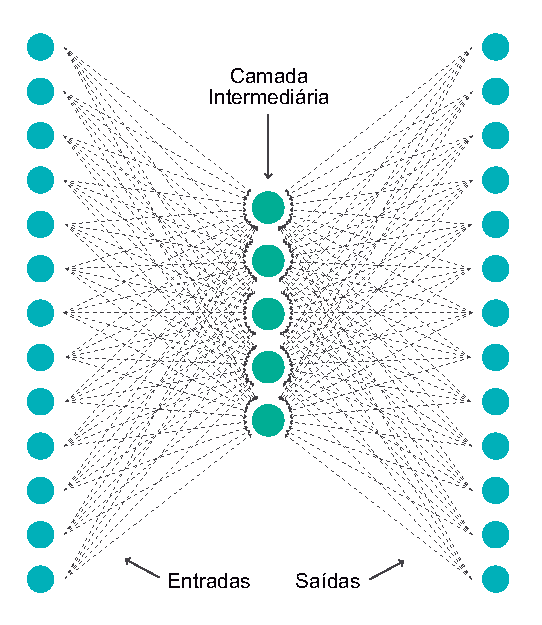
\includegraphics{04-Figuras/Arquitetura-AutoAssociativa}

\caption{Arquitetura da rede Competitiva Auto Associativa}

\label{figura:arquiteturaAuto}

\end{figure}